\chapter[SCP-049 疫医]{
    SCP-049 Plague Doctor\\
    SCP-049 疫医
}

\label{chap:SCP-049}

\begin{figure}[H]
    \centering
    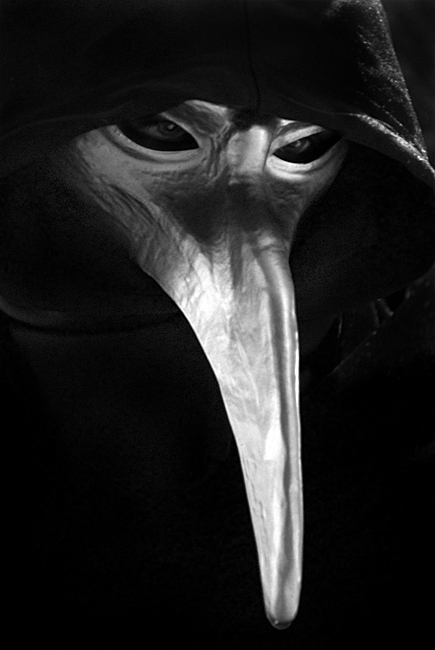
\includegraphics[width=0.5\linewidth]{images/SCP-049.jpg}
    \caption*{SCP-049,具有和人类高度相似的眼睛。}
\end{figure}

\bb{项目编号:}SCP-049

\bb{项目等级:}Euclid

\bb{特殊收容措施:}SCP-049须被看管于研究扇区-██的一个安全的隔间内。禁止将SCP-049从隔间内带离,除非有一个二级以上人员的许可,并且带离之前SCP-049必须实施重度镇定措施。即使如此,在移送SCP-049时还须有两个武装守卫陪同,以一个与两根2米长的铁竿绑定的铁箍引导,铁竿须掌握在两个一级以上人员的手上。对SCP-049进行的任何实验都必须在特殊准备的房间内进行。(见文档042-D-3-18)

SCP-049的隔间必须时刻被安保摄像机监控。若发生任何异变,须第一时间警告████医生。

\bb{描述:}SCP-049外表呈人形,站高1.9米体重95.3千克。然而,由于它身被一套15-16世纪欧洲传统的“黑死病医生”装束,基金会现在无法进一步研究它的脸部和身体。这套装束事实上是SCP-049身体的一部分,显微镜观察和基因测试显示其结构类似肌肉,虽然衣物部分感觉更像粗皮革且面具更像是陶制。它最初在英格兰,██████被当地警察发现。 机动特遣队{[}删除]就一次{[}资料删除]的疑似爆发作出响应。作为初期收容措施,已对半公里半径范围内的所有平民进行A级记忆消除。

\dd{SCP-049从不说话} (见附录A-1),尽管它看起来能毫无障碍地理解英语,并且它完全温和驯服,除非它试图进行外科手术。SCP-049的触碰对人类及其致命。碰触到SCP-049的手之后,受害人(以下称为SCP-049-2)会{[}数据删除]并且迅速死去。其后为了不受阻碍的回到SCP-049-2身边SCP-049会试图以相似的手法杀死目所能及的所有人。它会从体内的某个地方生成一个{[}数据删除]材质的手术包,内含外科手术刀,针线,和数瓶成分至今未知的药水(X光照射和类似技术无法确认这些工具在SCP-049体内的具体位置),开始解剖SCP-049-2并向其体内注射多种化学药品。经过约20分钟,SCP-049会将SCP-049-2缝合,重归驯服。

几分钟之后SCP-049-2会恢复生命迹象重新开始活动。然而SCP-049-2完全失去了高级大脑功能,并且会漫无目的的游荡直到遇到其他活人。此时SCP-049-2的肾上腺素及内啡肽水平会上升大约百分之三百(300),试图杀死并██████所有能找到的人类,然后重新开始无脑游荡直到再度遇到其他人类。在此阶段允许进行毫无怜悯的抹消。在实验以外的场合未能执行此程序(见附录T-049-12)者将可能被处决。

通过对SCP-049-2的尸检,在体内发现了数种异常物质(和大量正常物质一起),包括{[}数据删除]。一些物质仍待鉴别中。(3级及更高级别研究人员可参阅附录C-1)

\bb{附录A-1:}12-6-20██,今日SCP-049第一次开口说话,对象是Dr. ████。对话的完整记录如下。

\bb{询问:} SCP-049\\
\bb{询问者:}███████ ████博士\\
\bb{前言:}在前往一个实验设施的途中SCP-049在没有明显外部刺激的情况下突然开口说话。当时████医生通过一个手持麦克风记录了谈话。无关内容忽略。

\begin{scpbox}

SCP-049:这是个哪儿啊?\\
Dr. ████:啥?这是个实验……{[}传来一阵撞击声,因为████医生在震惊中扔掉了录音装置]\\
SCP-049:一个实验室?真神奇啊。怪不得你们这儿病人这么少。\\
Dr. ████:啊……啊。你看,我不知道你能讲话。我有点惊奇你,呃,能说话。\\
SCP-049:嗷,是的,对,好先生。我只是不想说罢了。大部分病人都很令人悲痛并且对谈话没啥反应。现在我观察了你几次,并且没在你身上看到染病的迹象,所以我估摸着你大概也是个医生?\\
Dr. ████:是的,是。叫我{[}改写]……话说回来你说的是什么疾病?\\
SCP-049:咋啦,好医生,当然是大瘟疫啦。还能是个啥病?\\
Dr. ████:大瘟……哦,传染病(应特指黑死病\slash 腺鼠疫;译注)。我应该知道有这么一出。不过没人被感染,我向你保证。\\
SCP-049:喔,好医生,我也向你保证,瘟疫就在这里,我能感觉到!使世界摆脱它的威胁是我毕生的职责。我的治疗最有效啦。\\
Dr. ████:你的治疗?你治死我们上百人!你的治疗是个灾难!\\
SCP-049:好医生,我的治疗是最有效的……

SCP-049重归沉寂,使之开口说话的进一步尝试皆不起作用。

\end{scpbox}

\bb{结语:}我们设法结束了那天的实验,并试图找出它实行外科手术的原因,或者更准确的,它所说的“瘟疫”是什么。至今为止研究表明它曾经实施过手术的D级人员间没有任何联系。我们还在继续研究。\\
████博士

\bb{附录C-1:需三级以上权限:}于4-26-20██,SCP-049设法逃出了收容。在脱离监视约5分钟后,它与SCP-███发生了接触。在被拘禁时,SCP-049表现十分友善平静,但是,直到目前为止,SCP-049在引发并进行手术时显得更为健谈。

\ii{我不知道那零四九和那该死的面具谈过了些什么,但他似乎是更高兴了。他似乎不再在舱间里闷闷不乐地静坐,而且有好些员工声称有听到他在哼唱著古老的教堂赞美诗。此外,在引发并进行手术的时候,他开始说话了,似乎是在….安抚他的受害者。声称他就是“\overtextnote{解药(cure)}”之类的。我们的研究资源已经转移至找出他和{[}删除]在那次小会面中到底聊了些什么鬼东西。 -████博士}
